\documentclass[12pt]{amsart}
\usepackage[letterpaper, portrait, left = 1in, right = 1in, top = 1.2in, bottom=1.5in]{geometry} 
%\usepackage{setspace} \doublespacing
%\usepackage[letterpaper, portrait, margin=1.3in]{geometry}
\usepackage[table,xcdraw]{xcolor}
\usepackage{amssymb}
\usepackage{amsfonts}
\usepackage{longtable}
\usepackage{amsmath,amsthm}
\usepackage{enumitem}
\usepackage[utf8]{inputenc}
\usepackage{mathtools}
\usepackage{graphicx}
\usepackage{parskip}
\usepackage{multicol}
\usepackage{listings}
\usepackage[skip=0.25pt]{caption}
\usepackage[mathscr]{euscript}
\usepackage{quiver}
\setlength{\parindent}{0pt}
\usepackage{thm-restate}
\definecolor{vividburgundy}{rgb}{0.62, 0.11, 0.21}
\usepackage[driverfallback=hypertex,pagebackref=false,colorlinks,citecolor=vividburgundy]{hyperref}
\usepackage[capitalize]{cleveref}
%\usepackage[cmintegrals,cmbraces]{newtxmath}
%\usepackage{ebgaramond-maths}

%\usepackage{fourier}
%----------FONT OPTIONS----------
% sans-serif
%\usepackage[sfdefault]{FiraSans}
 %\usepackage[sfdefault]{roboto}
% \usepackage[sfdefault]{noto-sans}
%\usepackage[default]{sourcesanspro}

% serif
%\usepackage{CormorantGaramond}

%\usepackage{charter}
\usepackage[T1]{fontenc}
\usepackage{cleveref}
\definecolor{dg}{RGB}{10, 100, 10}
\setlength{\parindent}{0in}
\renewcommand{\qed}{$\hfill\blacksquare$}
% \newtheoremstyle{style}{2pt}{1pt}{\normalfont}{}{\bfseries}{\\}{0cm}{}
% \theoremstyle{style}
\newtheorem{lemma}{Lemma}[section]
% \newtheorem{lemma}{Lemma}
\newtheorem{thm}[lemma]{Theorem}
\newtheorem{prop}[lemma]{Proposition}
\newtheorem{cor}[lemma]{Corollary}
\newtheorem{conj}[lemma]{Conjecture}
\newtheorem{cl}[lemma]{Claim}
\newtheorem{rmk}{Remark}
\newtheorem{defn}[lemma]{Definition}
\newtheorem{qs}{Question}
\newtheoremstyle{styleS}{}{}{\color{dg}}{}{\color{dg}\bfseries}{. }{0cm}{}
\theoremstyle{styleS}
\newtheorem*{sol}{Solution}
\newtheoremstyle{style1}{}{}{\normalfont}{}{\bfseries}{. }{0cm}{}
\theoremstyle{style1}
\newtheorem{prob}{Problem}[section]
\newtheorem*{prb}{Problem}
\newtheoremstyle{style2}{1pt}{4pt}{\normalfont}{}{\itshape}{. }{0cm}{}
\theoremstyle{style2}
\newtheorem{ex}[lemma]{Example}
\newtheorem*{pf}{Proof}

\newcommand{\norm}[2]{
\left\lVert #1 \right\rVert_{#2}
}
\usepackage{mathrsfs}
%\usepackage[table,xcdraw]{xcolor}
\usepackage{booktabs}
\usepackage{tikz}
\usetikzlibrary{matrix}
\renewcommand{\l}{\ell}


\newcommand{\fA}{{\mathfrak{A}}}   \newcommand{\fB}{{\mathfrak{B}}}
\newcommand{\fC}{{\mathfrak{C}}}   \newcommand{\fD}{{\mathfrak{D}}}
\newcommand{\fE}{{\mathfrak{E}}}   \newcommand{\fF}{{\mathfrak{F}}}
\newcommand{\fG}{{\mathfrak{G}}}   \newcommand{\fH}{{\mathfrak{H}}}
\newcommand{\fI}{{\mathfrak{I}}}   \newcommand{\fJ}{{\mathfrak{J}}}
\newcommand{\fK}{{\mathfrak{K}}}   \newcommand{\fL}{{\mathfrak{L}}}
\newcommand{\fM}{{\mathfrak{M}}}   \newcommand{\fN}{{\mathfrak{N}}}
\newcommand{\fO}{{\mathfrak{O}}}   \newcommand{\fP}{{\mathfrak{P}}}
\newcommand{\fQ}{{\mathfrak{Q}}}   \newcommand{\fR}{{\mathfrak{R}}}
\newcommand{\fS}{{\mathfrak{S}}}   \newcommand{\fT}{{\mathfrak{T}}}
\newcommand{\fU}{{\mathfrak{U}}}   \newcommand{\fV}{{\mathfrak{V}}}
\newcommand{\fW}{{\mathfrak{W}}}   \newcommand{\fX}{{\mathfrak{X}}}
\newcommand{\fY}{{\mathfrak{Y}}}   \newcommand{\fZ}{{\mathfrak{Z}}}

\newcommand{\cA}{{\mathcal{A}}}   \newcommand{\cB}{{\mathcal{B}}}
\newcommand{\cC}{{\mathcal{C}}}   \newcommand{\cD}{{\mathcal{D}}}
\newcommand{\cE}{{\mathcal{E}}}   \newcommand{\cF}{{\mathcal{F}}}
\newcommand{\cG}{{\mathcal{G}}}   \newcommand{\cH}{{\mathcal{H}}}
\newcommand{\cI}{{\mathcal{I}}}   \newcommand{\cJ}{{\mathcal{J}}}
\newcommand{\cK}{{\mathcal{K}}}   \newcommand{\cL}{{\mathcal{L}}}
\newcommand{\cM}{{\mathcal{M}}}   \newcommand{\cN}{{\mathcal{N}}}
\newcommand{\cO}{{\mathcal{O}}}   \newcommand{\cP}{{\mathcal{P}}}
\newcommand{\cQ}{{\mathcal{Q}}}   \newcommand{\cR}{{\mathcal{R}}}
\newcommand{\cS}{{\mathcal{S}}}   \newcommand{\cT}{{\mathcal{T}}}
\newcommand{\cU}{{\mathcal{U}}}   \newcommand{\cV}{{\mathcal{V}}}
\newcommand{\cW}{{\mathcal{W}}}   \newcommand{\cX}{{\mathcal{X}}}
\newcommand{\cY}{{\mathcal{Y}}}   \newcommand{\cZ}{{\mathcal{Z}}}

\newcommand{\sA}{{\mathscr{A}}}   \newcommand{\sB}{{\mathscr{B}}}
\newcommand{\sC}{{\mathscr{C}}}   \newcommand{\sD}{{\mathscr{D}}}
\newcommand{\sE}{{\mathscr{E}}}   \newcommand{\sF}{{\mathscr{F}}}
\newcommand{\sG}{{\mathscr{G}}}   \newcommand{\sH}{{\mathscr{H}}}
\newcommand{\sI}{{\mathscr{I}}}   \newcommand{\sJ}{{\mathscr{J}}}
\newcommand{\sK}{{\mathscr{K}}}   \newcommand{\sL}{{\mathscr{L}}}
\newcommand{\sM}{{\mathscr{M}}}   \newcommand{\sN}{{\mathscr{N}}}
\newcommand{\sO}{{\mathscr{O}}}   \newcommand{\sP}{{\mathscr{P}}}
\newcommand{\sQ}{{\mathscr{Q}}}   \newcommand{\sR}{{\mathscr{R}}}
\newcommand{\sS}{{\mathscr{S}}}   \newcommand{\sT}{{\mathscr{T}}}
\newcommand{\sU}{{\mathscr{U}}}   \newcommand{\sV}{{\mathscr{V}}}
\newcommand{\sW}{{\mathscr{W}}}   \newcommand{\sX}{{\mathscr{X}}}
\newcommand{\sY}{{\mathscr{Y}}}   \newcommand{\sZ}{{\mathscr{Z}}}

\newcommand{\ta}{{\tilde{a}}}   \newcommand{\tb}{{\tilde{b}}}
\newcommand{\tc}{{\tilde{c}}}   \newcommand{\td}{{\tilde{d}}}
\newcommand{\te}{{\tilde{e}}}   \newcommand{\tf}{{\tilde{f}}}
\newcommand{\tg}{{\tilde{g}}}   
\newcommand{\ti}{{\tilde{i}}}   \newcommand{\tj}{{\tilde{j}}}
\newcommand{\tk}{{\tilde{k}}}   \newcommand{\tl}{{\tilde{l}}}
\newcommand{\tm}{{\tilde{m}}}   \newcommand{\tn}{{\tilde{n}}}
		         	\newcommand{\tp}{{\tilde{p}}}
\newcommand{\tq}{{\tilde{q}}}   \newcommand{\tr}{{\tilde{r}}}
\newcommand{\ts}{{\tilde{s}}}   
\newcommand{\tu}{{\tilde{u}}}   \newcommand{\tv}{{\tilde{v}}}
\newcommand{\tw}{{\tilde{w}}}   \newcommand{\tx}{{\tilde{x}}}
\newcommand{\ty}{{\tilde{y}}}   \newcommand{\tz}{{\tilde{z}}}

\newcommand{\red}{{\color{red}red}}
\newcommand{\blue}{{\color{blue}blue}}

\newcommand{\into}{\hookrightarrow}
\newcommand{\onto}{\twoheadrightarrow}
\newcommand\N{\ensuremath{\mathbb{N}}}

%\newcommand\L{\ensuremath{\mathbb{L}}}
\newcommand{\bP}{\mathbb{P}}
\newcommand\M{\ensuremath{\mathbb{M}}}
\newcommand\R{\ensuremath{\mathbb{R}}}
\newcommand\Z{\ensuremath{\mathbb{Z}}}
\renewcommand\O{\ensuremath{\emptyset}}
\newcommand\Q{\ensuremath{\mathbb{Q}}}
\newcommand\C{\ensuremath{\mathbb{C}}}
\newcommand{\K}{\ensuremath{\mathbb{K}}}
\newcommand\F{\ensuremath{\mathbb{F}}}
\newcommand{\aff}{\ensuremath{\mathbb{A}}}
\newcommand{\proj}{\ensuremath{\mathbb{P}}}
\newcommand{\dd}{\mathrm{d}}
\newcommand{\m}{\ensuremath{\mathfrak{m}}}
\newcommand{\p}{\ensuremath{\mathfrak{p}}}
\newcommand{\n}{\ensuremath{\mathfrak{n}}}
\renewcommand{\phi}{\varphi}
\renewcommand{\qedsymbol}{\ensuremath{\blacksquare}}
%\newcommand{\st}{\;|\;}
\newcommand{\st}{%
  \nonscript\;
  \ifnum\currentgrouptype=16
    \;\middle|\;
  \else
    \;|\;
  \fi
  \nonscript\;}
\newcommand{\ltr}{\par \noindent \framebox[1\width]{ $\implies$ } \hspace{.2cm}}
\newcommand{\rtl}{\par \noindent \framebox[1\width]{ $\impliedby$ } \hspace{.2cm} }
\newcommand{\abs}[1]{\left| #1 \right|}
\newcommand{\inner}[2]{\left\langle #1, #2 \right\rangle}
\newcommand{\E}[1]{\mathbb E\left[ #1 \right]}
\newcommand{\e}[1]{\exp\left( #1 \right)}
\renewcommand{\P}[1]{\mathbb P\left[ #1 \right]}
\newcommand{\Var}[1]{\text{Var}\left[ #1 \right]}
\newcommand*\circled[1]{\tikz[baseline=(char.base)]{
            \node[shape=circle,draw,inner sep=2pt] (char) {#1};}}
\newcommand{\ds}{\displaystyle}

\DeclareMathOperator{\sym}{Sym}
\DeclareMathOperator{\mds}{MDS}
\DeclareMathOperator{\Tor}{Tor}
\DeclareMathOperator{\Ext}{Ext}
\DeclareMathOperator{\adj}{adj}
\DeclareMathOperator{\Tr}{Tr}
\DeclareMathOperator{\GL}{GL}
%\DeclareMathOperator{\Tr}{Tr}
\DeclareMathOperator{\orbit}{Or}
\DeclareMathOperator{\stab}{Stab}
\DeclareMathOperator{\fix}{Fix}
\DeclareMathOperator{\re}{Re}
\DeclareMathOperator{\im}{Im}
\DeclareMathOperator{\ord}{Ord}
\DeclareMathOperator{\mspec}{mSpec}
\DeclareMathOperator{\spec}{Spec}
\DeclareMathOperator{\frob}{Frob}
\DeclareMathOperator{\id}{Id}
\DeclareMathOperator{\colim}{colim}
\DeclareMathOperator{\loc}{loc}
\DeclareMathOperator{\res}{Res}
\DeclareMathOperator{\rad}{rad}
\DeclareMathOperator{\Res}{Res}
\DeclareMathOperator{\diam}{diam}
\DeclareMathOperator{\arcsec}{arcsec}
\DeclareMathOperator{\arccot}{arccot}
\DeclareMathOperator{\len}{len}
\DeclareMathOperator{\area}{area}
\DeclareMathOperator{\vol}{vol}
\DeclareMathOperator{\ev}{ev}
\DeclareMathOperator{\sgn}{sgn}
\DeclareMathOperator{\supp}{supp}
\DeclareMathOperator{\diff}{d}
\DeclareMathOperator{\Dom}{Dom}
\DeclareMathOperator{\rk}{rank}
\renewcommand{\d}{\diff}
\let\oldend\endlinechar
\renewcommand{\endlinechar}{\oldend}
\newcommand{\open}{\underset{\text{open}}{\subset}}
\newcommand{\divides}{\mathbin{|}}
\newcommand{\set}[1]{\ensuremath{\left\{#1\right\}}}
\newcommand{\sett}{\coloneqq}
\newcommand*\isomap{%
  \xrightarrow{\raisebox{-0.9ex}[0ex][0ex]{$\sim$}}%
}
\renewcommand{\epsilon}{\varepsilon}
\newcommand{\fa}{~\forall~}
%\usepackage[nobottomtitles*]{titlesec}
\usepackage{titletoc}
%\titleformat{\section}[runin]
%{\normalfont\Large\bfseries}
%{}{0pt}{}%
%[\ifthenelse{\equal{\thesection}{0}}{\\\vspace*{0pt}}{\space\thesection}]
\newcommand{\sint}{\sin\theta}
\newcommand{\cost}{\cos\theta}
\newcommand{\tant}{\tan\theta}
\newcommand{\lb}{\left[}
\newcommand{\rb}{\right]}
\newcommand{\lp}{\left(}
\newcommand{\rp}{\right)}
\newcommand{\br}[1]{\lb#1\rb}
\newcommand{\pa}[1]{\lp#1\rp}
\usepackage{pdfpages}
\usepackage{fancyhdr}
	\pagestyle{fancyplain}
	\fancyhf{}
	\fancyhead[C]{\thepage}

\usepackage{wrapfig}
%\fontfamily{qcr}\selectfont 
%\usepackage[backend=bibtex]{biblatex}
\usepackage[
backend=biber,
style=alphabetic,%firstinits,
citestyle=ieee-alphabetic,
%natbib=true,
%uniquelist=false,
maxnames=10,
sorting=ynt
]{biblatex}
%\addbibresource{writeup/article/refs.bib}
%\title{\vspace{-1cm}}
\title{\textbf{CONVEX AND CONIC OPTIMIZATION}\\ Homework $1$}
\usepackage{quiver}
\usepackage[nobottomtitles*]{titlesec}
\usepackage{titletoc}
\titleformat{\section}[runin]
  {\normalfont\Large\bfseries}
  {}{0pt}{}%
  [\ifthenelse{\equal{\thesection}{0}}{\\\vspace*{0pt}}{\space\thesection}]
\author{{\Large NILAVA METYA} \\ 
\href{mailto:nilava.metya@rutgers.edu}{nilava.metya@rutgers.edu}\\
\href{mailto:nm8188@princeton.edu}{nm8188@princeton.edu}}
\date{February $27$, $2024$}
\newcommand{\pb}{\section{Problem}~\par}
\newcommand{\soln}{\subsection*{Solution}}
\newcommand{\conv}{\text{conv}}
\newcommand{\epi}{\text{epi}}
\usepackage{pdfpages}
\usepackage{fancyhdr}
	\pagestyle{fancyplain}
	\fancyhf{}
	\fancyhead[R]{\thepage}
\setlength{\columnsep}{1.2cm}
\begin{document}

\maketitle

%$\boxed{
%B(x,r), B^o(x,r) \text{ respectively denote the closed and open balls of radius } r \text{ around }x.}$

\pb
Let $S\subseteq\R^{n}$.
\begin{enumerate}[leftmargin=*]
\item The convex hull of S is the intersection of all convex sets that contain S.
\item If $S$ is closed, then the convex hull of $S$ is closed.
\item If $S$ is bounded, then the convex hull of $S$ is bounded.
\item If $S$ is compact, then the convex hull of $S$ is compact.
\item The sum of two quasiconvex functions is quasiconvex.
\item A quadratic function $f(x) = x^{\top} Qx + b^{\top} x + c$ is convex if and only if it is quasiconvex.
\item Any closed convex set $\Omega\subseteq \R^{n}$ can be written as $\Omega=\set {x\in \R^{n}\st g(x)\le 0}$ for some convex function $g : \R^{n} \to \R$.
\item If $f : \R^{n} \to \R$ is convex on a convex set $S \subseteq \R^{n}$, then $f$ is continuous on $S$.
\item Suppose $P \in \R^{n\times n}$ is a matrix with nonnegative entries whose columns each sum up to one. Then, there exists $x\in \R^{n}$ such that $Px=x,x\ge0$,and $\sum_{i}x_{i}=1$.
\item A continuous function $f:\R^{n}\to\R$ satisfying the midpoint convexity property $$f\left(\frac{x+y}{2}\right) \leq \frac{f(x)+f(y)}{2}\forall x,y\in\R^{n}$$ is convex.
\end{enumerate}

\soln

\begin{enumerate}[leftmargin=*]
\item  \textbf{True}.

Let $\cC=\conv(S)$ as defined in class (collection of convex combinations) and let $\cX$ be the intersection of all convex sets that contain $S$. \\It is clear that $S\subseteq \cC$ whence $\boxed{\cX\subseteq \cC}$ by the description of $\cX$. \\Now, if $T$ is a convex set containing $S$, then any convex combination $x$ of points in $S$ is a convex combination of points in $T$, so $x\in T$. This shows that $\cC\subseteq T$. Again by description of $\cX$, we have $\boxed{\cC\subseteq \cX}$.

\item \textbf{False}.

\begin{multicols}{2}
Consider $S = \set{(x,y)\in\R^{2}\st y\ge e^{-\abs x}}$. We'll show that $\cC\sett\conv (S)$ is $\cX\sett\set{(x,y)\in\R^{2}\st y>0}$. Clearly $S\subseteq\cX$ because exponential takes only positive values, so $\boxed{\cC=\conv(S)\subseteq \conv(\cX) = \cX}$, where the last equality is true because $\cX$ is convex (if two points have positive $y-$coordinate, so do their convex combinations). \\On the other hand, say $(a,b)\in\cX$, pick a large enough $\theta$ such that $\min(\abs{a+\theta}, \abs{a-\theta}) > \ln\frac1b$. This ensures that $e^{-\abs{a\pm\theta}} < b$ so that $(a\pm\theta,b)\in S$ and thus their average $(a,b)\in \cC$. This proves that $\boxed{\cX\subseteq \cC}$. \\
So $\cX = \conv(S)$ where $S$ is closed but $\cX$ (the strict upper half plane) is not.


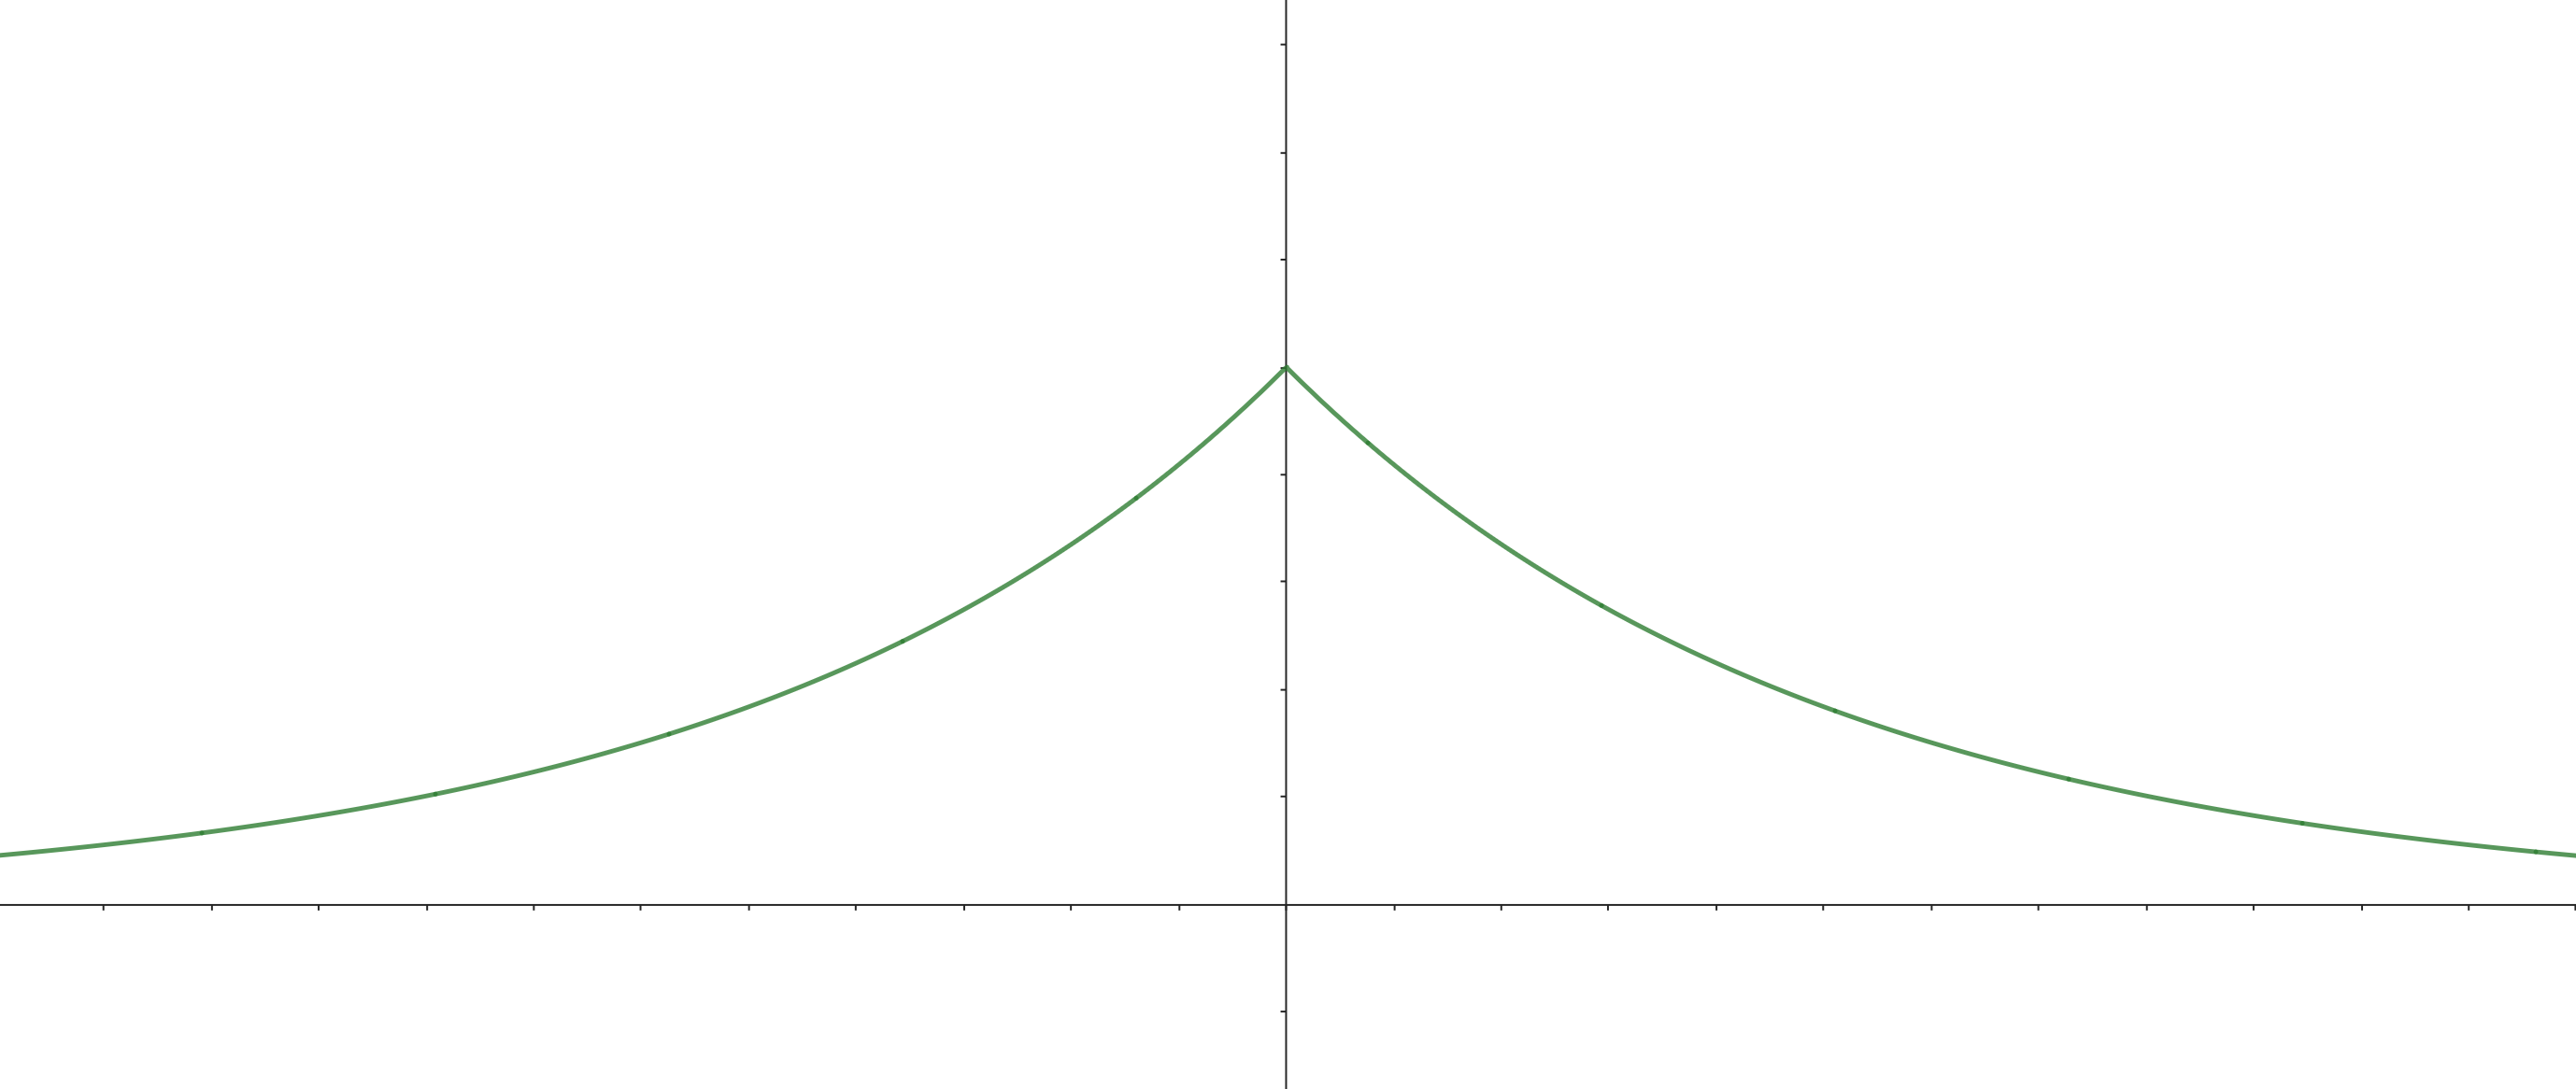
\includegraphics[width=0.45\textwidth]{closed.png}
\captionof*{figure}{$S$ is the epigraph of this function}
\end{multicols}

\item \textbf{True}.

$S$ is bounded, so $\exists\delta>0$ such that $S\subseteq B(0,\delta)$. Recall that $B(0,\delta)$ is convex. This implies that $\conv(S)\subseteq \conv(B(0,\delta)) = B(0,\delta)$, whence $\text{conv}(S)$ is bounded.
\item \textbf{True}.

We'll use the fact that a set in Euclidean space is compact iff it is sequentially compact. We say that a set $T$ is sequentially compact if every sequence of points in $T$ has a convergent subsequence (with limit in $T$). $\boxed{\text{We will use a}\bullet \text{ in subscript to suppress the lower index of a sequence}.}$\\
Assume $S$ is compact (hence sequentially compact). It is also important to note that $[0,1]$ is (sequentially) compact. Consider a sequence of points $\set{a_{k}}_{{k\in\N}}$ in $\conv(S)$. By Caratheodory's theorem, for each $a_{k}$, there are $n+1$ non-negative reals $\lambda^{(k)}_{1},\cdots,\lambda^{(k)}_{n+1}\in[0,1]$ adding to $1$ and $n+1$ points $x^{(k)}_{1}, \cdots,x^{(k)}_{1}\in S$ such that $\ds a_{k} = \sum_{i=1}^{n}\lambda^{(k)}_{i}x^{(k)}_{i}$ (I want to emphasize again that this is for each $a_{k}$). \\
Consider the sequence $\set{\lambda^{(1)}_{k}}_{k\in\N}$. This is a sequence in the compact unit interval and thus has a convergent subsequence, say $\set{\lambda^{(1)}_{d^{(1)}_{k}}}_{k\in\N}$. Let the limit of this subsequence be $\lambda^{(1)}$. Next note that $\ds\set{x^{(1)}_{d^{(1)}_{k}}}_{k\in\N}$ is a sequence in the compact set $S$ and thus has a convergent subsequence, say $\set{x^{(1)}_{\td^{(1)}_{k}}}_{k\in\N}$. So $\set{\td^{(1)}_{k}}_{k\in\N}$ is a subsequence of $\set{d^{(1)}_{k}}_{k\in\N}$, and thus does not affect the convergence of $\lambda^{(1)}_{\td^{(1)}_{k}}$. Let the limit of $\set{x^{(1)}_{\td^{(1)}_{k}}}_{k\in\N}$ be $x^{(1)}\in S$. Notice that $\ds\lim_{{k\to\infty}}\lambda^{(1)}_{\td^{(1)}_{k}}x^{(1)}_{\td^{(1)}_{k}} = \lambda^{(1)}x^{(1)}$, which happens because
\begin{align*}\ds\norm{\lambda^{(1)}_{\td^{(1)}_{k}}x^{(1)}_{\td^{(1)}_{k}} - \lambda^{(1)}x^{(1)}}{}
&\leq \norm{\lambda^{(1)}_{\td^{(1)}_{k}}x^{(1)}_{\td^{(1)}_{k}} - \lambda^{(1)}_{\td^{(1)}_{k}}x^{(1)}}{} + \norm{\lambda^{(1)}_{\td^{(1)}_{k}}x^{(1)} - \lambda^{(1)}x^{(1)}}{}\\
&= \lambda^{(1)}_{\td^{(1)}_{k}}\underbrace{\norm{x^{(1)}_{\td^{(1)}_{k}} - x^{(1)}}{}}_{\text{can be made arbitrarily small}} + \underbrace{\abs{\lambda^{(1)}_{\td^{(1)}_{k}} - \lambda^{(1)}}}_{{\text{can be made arbitrarily small}}} \norm{x^{(1)}}{}.
\end{align*}
By following a similar procedure, one can further extract a subsequence $\set{d^{(2)}_{k}}_{k\in\N}$, which makes $\lambda^{(2)}_{\bullet}$ converge to $\lambda^{(2)}$, and a further sub-subquence $\set{\td^{(2)}_{k}}_{k\in\N}$ which makes $x^{(2)}_{\bullet}$ converge to $x^{(2)}$. Note that this smaller sequence does not affect the convergence of $\lambda^{(1)}_{\bullet}$ and $x^{(1)}_{\bullet}$ (and also their product). By the same argument as above, $\ds\lim_{{k\to\infty}}\lambda^{(2)}_{\td^{(2)}_{k}}x^{(2)}_{\td^{(2)}_{k}} = \lambda^{(2)}x^{(2)}$. \\
We do this (extracting subsequences in turn for convergence of subsequences of $\lambda^{(1)}_{\bullet},x^{(1)}_{\bullet},\lambda^{(2)}_{\bullet}, x^{(2)}_{\bullet}, \lambda^{(3)}_{\bullet},\cdots$) for a total of $n+1$ times, and finally get a subsequence $\set{\td^{(n+1)}_{k}}_{{k\in\N}}$ which ensures convergence of $\lambda^{(i)}_{\td^{(n+1)}_{k}}\xrightarrow{k\to\infty} \lambda^{(i)}$ and $x^{(i)}_{\td^{(n+1)}_{k}}\xrightarrow{k\to\infty} x^{(i)}$ for every $i=1,\cdots,n+1$. It thus stands that $\lambda^{(i)}\in[0,1]$, $ x^{(i)}\in S\forall i$ and $\ds\sum_{i=1}^{n+1}\lambda^{(i)} = \sum_{i=1}^{n+1}\lim_{{k\to\infty}}\lambda^{(i)}_{\td^{(n+1)}_{k}} = \lim_{{k\to\infty}}\sum_{i=1}^{n+1}\lambda^{(i)}_{\td^{(n+1)}_{k}} = \lim_{{k\to\infty}} 1 = 1$ where the sum and limit could be exchanged because each limit exists. Thus $\set{a_{\td^{(n+1)}_{k}}}_{k\in\N}$ is a subsequence of $\set{a_{k}}_{k\in\N}$ which converges to $\ds a\sett \sum_{i=1}^{n+1}\lambda^{(i)}x^{(i)}$. $a\in \conv(S)$ because each $x^{(i)}\in S$ by construction and the $\lambda^{(i)}$'s form a convex weight for the $x^{(i)}$'s.

\item \textbf{False}.

Consider $f(x) = x^{3}, g(x) = x^{2}$. Then $f$ is quasiconvex with sublevel sets $S_{\alpha}(f) = \left(-\infty,\alpha^{\frac13}\right]$ and $g$ is quasiconvex with sublevel sets $S_{\alpha}(g) = \begin{cases}\left[-\sqrt\alpha,\sqrt\alpha\right] &\text{if }\alpha \geq 0\\\varnothing&\text{otherwise}
\end{cases}$. But $(f+g)(x) = x^{3}+x^{2}$ is not quasiconvex. Indeed, $f+g\leq 0\iff x^{2}(x+1)\leq 0\iff x=0\text{ or } x \leq -1$, so $S\sett S_{0}(f+g) = (-\infty,-1]\cup \set{0}$ which is not convex because $\frac{-1+0}{2} = \frac{-1}{2}\notin S$ even though $0,-1\in S$.

\item \textbf{True}.

We already know convexity implies quasiconvexity. We'll prove the (contrapositive of) converse for quadratic polynomals (that is, not convex implies not quasiconvex). Note here that convexity is same as midpoint convexity by problem 1(10) because quadratic polynomials are continuous. Problem 1(10) can be used because this probem has not been used there and thus there is no circular argument.\\
$f(x) = x^{\top} Q x + b^{\top}x + c$, where $Q$ is symmetric (WLOG). Assume that $f$ is not convex. So $\exists x,y\in\R^{n}$ such that 
\begin{align*}
f\left(\frac{x+y}{2}\right) &> \frac{f(x)+f(y)}{2}\\
\implies \frac{1}{2}(x+y)^{\top}Q(x+y) + {\color{red}b^{\top} (x+y)} &> x^{\top}Qx + y^{\top}Qy + {\color{red}b^{\top} (x+y)}\\
\implies x^{\top}Qx + y^{\top}Qy + 2 x^{\top}Qy &> 2\left(x^{\top}Qx + y^{\top}Qy\right)\\
\implies x^{\top}Qx + y^{\top}Qy + 2 x^{\top}Qy &< 0\\
\implies (x-y)^{\top}Q(x-y) &< 0
\end{align*}
Let $z = \begin{cases}x-y &\text{if } b^{\top}(x-y)\ge 0\\ y-x&\text{otherwise}\end{cases}$. So this ensures that $B\sett b^{\top} z\ge 0$ and $A\sett z^{\top}Qz<0$. Note that $B^{2}-4A = B^{2}+4\abs A>0$ so that $\ds \lambda_{\pm}\sett \frac{-B\pm\sqrt{B^{2}-4A}}{2A}$ are well defined real numbers. These are precisely the roots of the polynomial $At^{2}+Bt+1=0$. We thus note that $f(\lambda_{\pm} z) = \lambda_{\pm}^{2}A + \lambda_{\pm} B + c = c-1$. Consider the sublevel set $S\sett S_{c-1} = \set{q\in \R^{n}\st f(q)\leq c-1}$. We've shown that $p_{1}\sett\lambda_{+} z, p_{2}\sett\lambda_{-} z\in S$ because $f(p_{1}) = f(p_{2}) = c-1$. But $\ds \frac{p_{1}+p_{2}}{2} = \frac{\lambda_{+}z + \lambda_{-}z}{2} = \frac{-B}{2A}z$ whence \begin{align*}
f\left(\frac{p_{1}+p_{2}}{2}\right) &= f\left(\frac{-B}{2A}z\right)\\
&= \frac{B^{2}}{4A^{2}}A - \frac{B}{2A}B + c\\
&= \frac{B}{4(-A)} + c \ge c \\
&> c-1 \\
\implies \frac{p_{1}+p_{2}}{2} &\notin S.
\end{align*}
This proves that $S$ is not convex. So $f$ is not quasiconvex.


\item \textbf{True}.

$\Omega$ is closed and convex. For each $x\in \R^{n}$ there is a point $p^{*}\in \Omega$ such that $\ds\inf_{p\in \Omega} \norm{x-p}{} = \norm{x-p^{*}}{}$. This is because the optimal value of $\ds\inf_{p\in \Omega} \norm{x-p}{}$, for a fixed $x$, is same as that obtained by optimizing over $\Omega\cap B(x,R)$ for some large enough radius $R$ such that $B(x,R)\cap \Omega$ is nontrivial (this intersection is closed and bounded and thus there is an optimal solution). \\
Consider the function $g:\R^{n}\to \R$ given by $g(x) = \ds\inf_{p\in \Omega}\norm{x-p}{}$. Then $g$ is convex. Indeed, if $u,v\in \R^{n}$ and $\lambda\in[0,1]$ then there are points $a,b\in \Omega$ such that $g(u) = \norm{u-a}{}, g(v) = \norm{v-b}{}$, which means that \begin{align*}
\lambda g(u) + (1-\lambda)g(v) &= \lambda\norm{u-a}{} + (1-\lambda)\norm{v-b}{} \\
&\ge \norm{\lambda u + (1-\lambda)v - \underbrace{\left[\lambda a + (1-\lambda)b \right]}_{\in \Omega}}{} \\
&\ge \ds\inf_{p\in \Omega}\norm{\lambda u + (1-\lambda)v-p}{} = g(\lambda u + (1-\lambda)v).
\end{align*}
We will show that $\Omega = \set{x\in\R^{n}\st g(x)\le 0}$. By definition, $g(x) = 0\forall x\in\Omega$, so $\Omega\subseteq \set{x\in\R^{n}\st g(x)\le 0}$. For the other inclusion, observe that if $g(x)\le 0$ then $g(x)=0$ because $g$ is the infimum over norms, hence non-negative, so that $\norm{x-p^{*}}{} = 0$ (where $p^{*}\in\Omega$ is the optimal solution for the abovementioned optimization problem). This means $x=p^{*}\in \Omega$. So the other inclusion is also true.


\item \textbf{False}.

The counterexample is obtained by taking $S=[0,1]\subseteq \R$ and $f(x) = \pmb 1_{x=1} = \begin{cases}
0 & \text{if } 0\leq x < 1\\
1 & \text{otherwise}
\end{cases}$. In each dimension, there is a counterexample, namely $S=[0,1]^{n}\subseteq\R^{n}$ and $f=\pmb 1_{x=(1,\cdots,1)}$. $S$ is clearly convex. The function is convex because it is constant $0$ except for one point and if $p=(1,\cdots,1)$ and $q\in S\smallsetminus \set{p}$ then for any $\lambda\in(0,1]$ we have $\lambda p + (1-\lambda)q\neq (1,\cdots,1)$ whence $f(\lambda p + (1-\lambda)q) = 0 \leq \lambda = \lambda f(p) + (1-\lambda)f(q)$. But clearly $f$ is not continuous.

\item \textbf{True}.

\textit{\textbf{First solution}:} (using Farkas lemma) \\
Consider $A=\begin{bmatrix}& &P\\1 & 1 & \cdots &1 \end{bmatrix} - \begin{bmatrix}&&\pmb 1_{{n\times n}}\\0 & 0 & \cdots &0 \end{bmatrix}\in\R^{(n+1)\times n}$, where $\pmb 1_{n\times n}$ is the $n\times n$ identity matrix, and $b = \begin{bmatrix}0\\\vdots\\0\\1\end{bmatrix}=f_{n+1}\in\R^{n+1}$ the $(n+1)^{\text{st}}$ basic vector in $\R^{n+1}$. Let $\ty = \begin{bmatrix}y_{1}\\\vdots\\y_{n}\\t\end{bmatrix}\in \R^{n}$ be an arbitrary real column vector. Consider the index $k\in\set{1,\cdots,n}$ such that $\ds y_{k} = \min_{i\le i\le n}y_{i}$. Then \begin{align*}
\left(A^{\top}\ty\right)_{k} &= \sum_{i=1}^{n} p_{ik}y_{i} - y_{k} + t\\
&= \sum_{i=1}^{n} p_{ik}y_{i} - \sum_{i=1}^{n} p_{ik}y_{k} + t &[\because\text{column sum }=1]\\
&= \sum_{i=1}^{n} p_{ik}(y_{i}-y_{k}) + t\\
&\ge t &[\because p_{ik}\ge 0, y_{i}-y_{k}\ge 0]\\
&= b^{\top}\ty
\end{align*}
This means $\set{\ty\st A^{\top}\ty\le 0, b^{\top}\ty >0} = \varnothing$ because $0\ge A^{\top}\ty\ge b^{\top}\ty >0$ is infeasible. By Farkas lemma, $\set{x\in\R^{n}\st Ax=b, x\ge 0}\ne \varnothing$. This simply means that there is a vector $x\in\R^{n}$ such that $(P-\pmb 1_{n\times n})x = 0$ (using the first $n$ rows of $A$) with the properties that $\ds\sum_{i}x_{i}=1$ (using last row of $A$) and $x\ge 0$

\textit{\textbf{Second solution}:} \\
We know that $P^{\top}\begin{bmatrix}1\\\vdots\\1\end{bmatrix} = \begin{bmatrix}1\\\vdots\\1\end{bmatrix}$ because each column of $P$ sums to $1$. Recall that row rank is same as column rank, whence $\rk (P-\pmb 1_{n\times n}) = \rk \left((P-\pmb 1_{n\times n})^{\top}\right) = \rk(P^{\top}-\pmb 1_{n\times n}) < n$. This means $\ker (P-\pmb 1_{n\times n}) \ne \set{0}$ and so there is some $v\in\R^{n}\smallsetminus\set{0}$ such that $Pv=v$. If each $v_{i}\ge 0$, our required vector is $\frac{v}{\norm v 1}$. If each $v_{i}\le 0$ we can take $x = \frac{-v}{\norm v 1}$ to ensure that $x_{i}\ge 0\forall i$ and $\sum x_{i}=1$. \\Assume otherwise, that is, some indices are positive, some are negative. Then consider $v^{+} = (v_{1}^{+},\cdots,v_{n}^{+})$ where $v_{i}^{+} = \max(0,v_{i})\ge 0$. This means $\ds(Av^{+})_{k} - (v)_{k} = (Av^{+} - v)_{k} = (A(v^{+}-v))_{k} \ge 0$ because $v^{+}-v\ge 0$ and $A$ has nonnegative entries, so $Av^{+}\ge v$. But $Av^{+}\ge 0$ because $A,v^{+}$ all have non-negative entries. This proves $Av^{+}- v^{+}\ge0$. But $\begin{bmatrix}1\\\vdots\\1\end{bmatrix}^{\top} Av^{+} = \begin{bmatrix}1\\\vdots\\1\end{bmatrix}^{\top} v^{+} $ by associativity, whence $\begin{bmatrix}1\\\vdots\\1\end{bmatrix}^{\top}(Av^{+}-v^{+}) = 0$ where the LHS is the sum of entries of the non-negative vector $Av^{+}-v^{+}$. This can only happen when each entry of $Av^{+}-v^{+}$ is $0$. This shows $Av^{+}=v^{+}$. So we are done by taking $x=\frac{v^{+}}{\norm{v^{+}}1}$ because $v^{+}$ is a nonzero vector because of our assumptions.

\item \textbf{True}.

Say $f$ is midpoint convex (that is, satisfies the given condition). \\
Consider $\epi(f) = \set{(x,t)\in \R^{n}\times\R\st f(x)\leq t}$. Consider a sequence $\set{(x_{n},t_{n})}_{n\in\N}$ of points in $\epi(f)$ that converge to $(a,s)\in \R^{n}\times\R$. This implies $\ds\lim_{n\to\infty} x_{n} = a, \lim_{n\to\infty} t_{n}=s$. By choice of points, $\ds t_{n}\ge f(x_{n})$ whence $\ds \lim_{n\to\infty} t_{n}\ge \lim_{n\to\infty} f(x_{n}) \stackrel{f \text{ continuous}}{=} f(a)$. By definition, $(a,s)\in\epi(f)$. Thus, $\epi(f)$ is closed. \\
Say $(x,t),(y,u)\in\epi(f)$. So $u\geq f(y), t\geq f(x)$. Then by midpoint convexity of $f$, we have $f\left(\frac{x+y}{2}\right) \leq \frac{f(x)+f(y)}{2} \leq \frac{u+t}{2}$ and, by definition of $\epi(f)$, this implies $\left(\frac{x+y}{2},\frac{u+t}{2}\right)\in \epi(f)$. So $\epi(f)$ is mid-point convex.\\
Since $\epi(f)$ is closed and midpoint convex, $\epi(f)$ is convex. This implies $f$ is convex.
\end{enumerate}

\newpage

\pb

\soln


\textit{\underline{Explanation:}}

First note that $\ds x(N) = \sum_{i=0}^{N-1}u(i)A^{N-1-i}b = \underbrace{\begin{bmatrix}A^{N-1}b & A^{N-2}b & \cdots & Ab & b\end{bmatrix}}_{M}\begin{bmatrix}u(0)\\\vdots\\u(N-1)\end{bmatrix}$. Thus one constraint must be $\boxed{Mu = x_{\text{des}}}$, which is linear. 

We want to solve \[\begin{aligned}
\min_{u} &\sum_{i=0}^{N-1} f(u(i))\\
\text{s.t. } 
&M u = x_{\text{des}}
\end{aligned}\]


Next note that $f(a)=\max\left(\abs a, 2\abs a-1\right)$. There are two issues to address while forming affine constraint(s): one is the absolute value, another is the $\max$ function. The first one is addressed by considering a variable $v(i)\ge0$ for each $i\in\set{0,1,\cdots,N-1}$, such that $\boxed{u(i)\le v(i)}$ and $\boxed{-u(i)\le v(i)}$ and taking the tightest such $v(i)$, so the objective function might be written as a minimization of these $\ds\sum_{i=0}^{N-1}f(v(i)) = \sum_{i=0}^{N-1}\max\left(v(i),2v(i)-1\right)$. But now the objective isn't affine. We can further introduce a variable $w(i)$ for each $i$ that satisfies $\boxed{w(i)\ge v(i)}$ and $\boxed{w(i)\ge 2v(i)-1}$, which ensures that $w(i)\ge f(v(i))$ and minimizing $w(i)$ ensures that the optimal value is indeed $f(v(i))$.
\\

\textit{\underline{The LP formulation:}}

So we propose the following LP:
\[\begin{aligned}
\min_{u,v,w} &\sum_{i=0}^{N-1} w(i)\\
\text{s.t. } 
&M u = x_{\text{des}}\\
&-v+u\le 0\\
&-v-u\le 0\\
&-w+v\le 0\\
&2v-\pmb c -w\le 0
\end{aligned}\]
where $\pmb c$ is the column vector of length $N$ containing all $1$'s. 


See code next page onwards


%\textit{\underline{Proving equivalence:}}
%
%Our intended problem was 
%\begin{align*}
%\min &\sum_{i=0}^{N-1} \max\left(\abs{u(i)}, 2\abs{u(i)}-1\right)\\
%\text{s.t. } 
%&M u = x_{\text{des}}.
%\end{align*}
%Call this problem $(2)$.
%
%Suppose $(u^{*},v^{*},w^{*})$ is a solution to $(1)$, then we will show that $u^{*}$ is a solution to $(2)$. Here $u^{*},v^{*},w^{*}\in\R^{N}$. Clearly $u^{*}$ satisfies $Mu^{*}=x_{\text{des}}$, so $u^{*}$ is feasible to $(2)$.
%
%
%We'll first prove a lemma
%\begin{lemma}
%Say $\Omega\subseteq \R$ and $g:\Omega\to \R$ is a non-decreasing function, that is, if $x,y\in\Omega$ are such that $x\ge y$ then $g(x)\ge g(y)$. Then the optimization problem 
%$$\begin{aligned}
%\min_{x\in\R^{n}} & \sum_{i=1}^{n} g(\max(\alpha(x_{i}),\beta(x_{i})))\\
%\textrm{s.t.} & 
%\end{aligned}$$
%\end{lemma}

{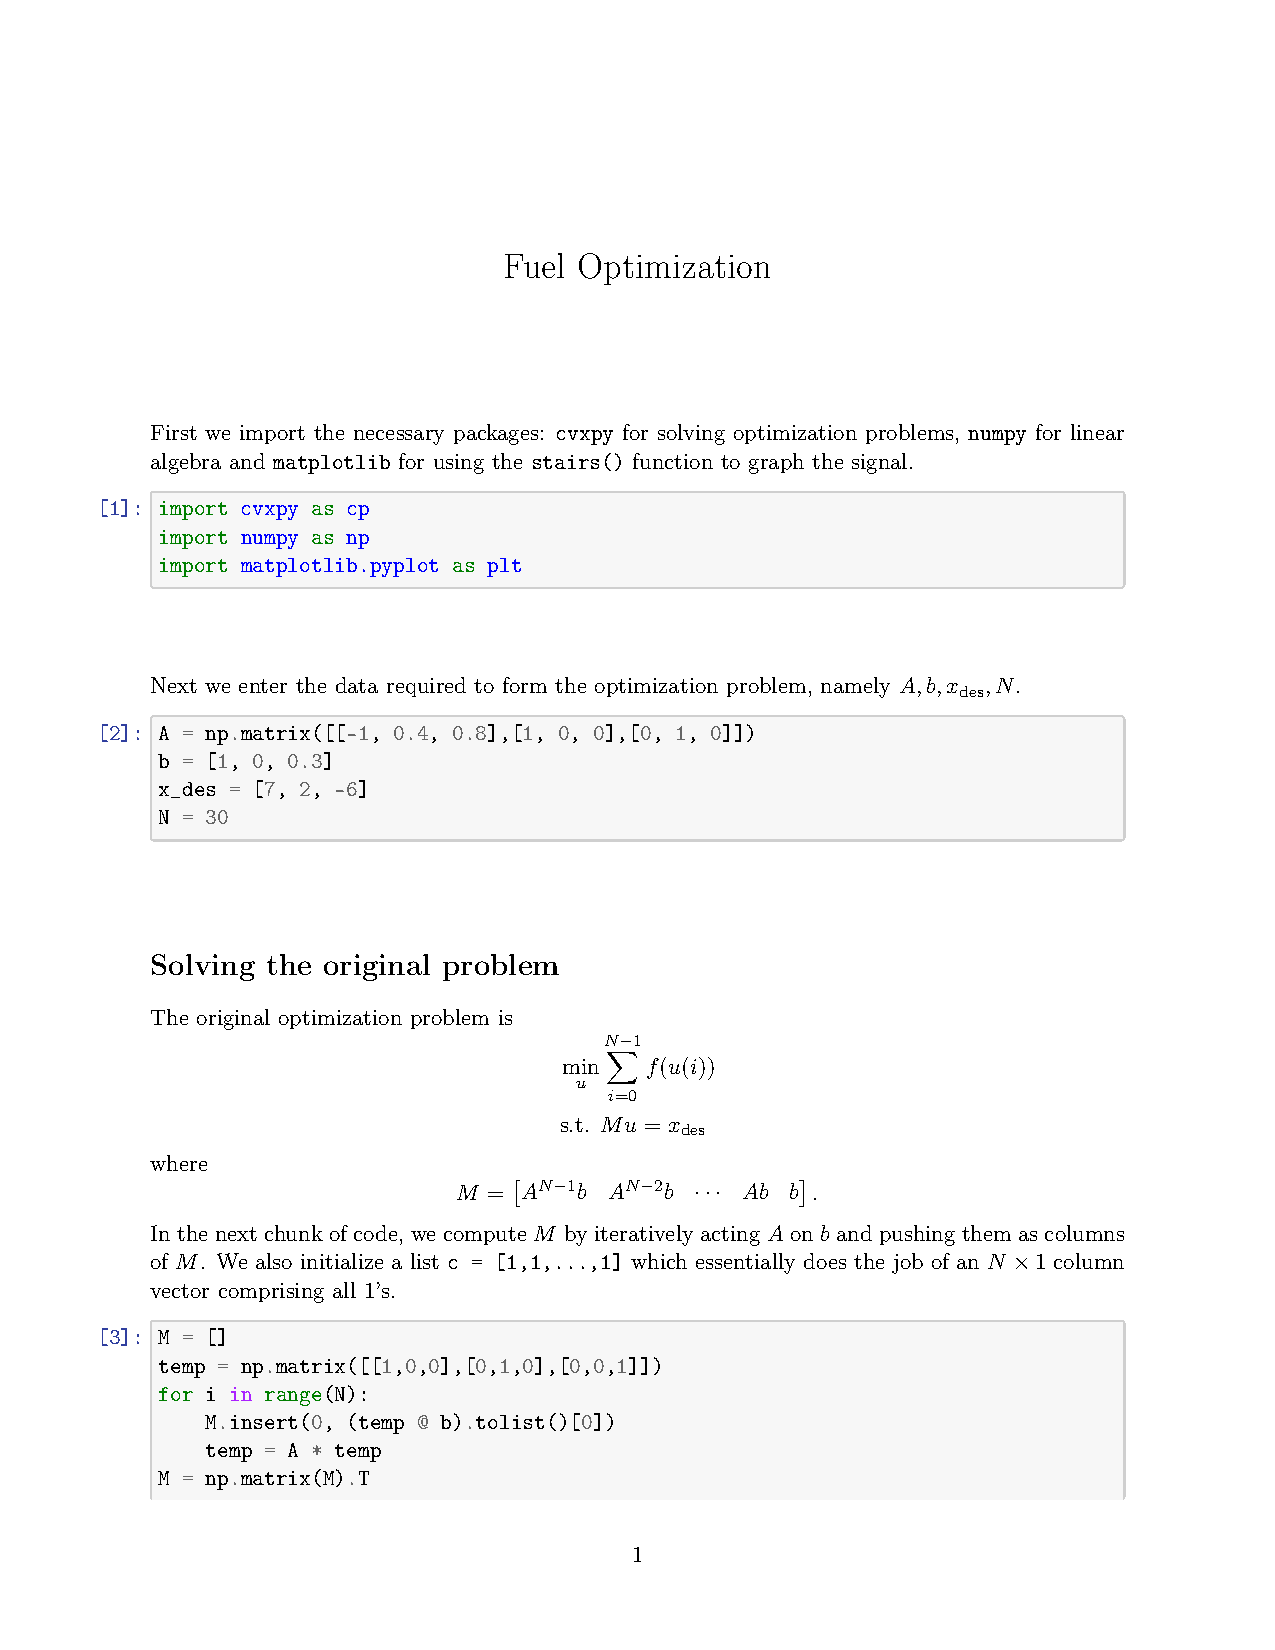
\includepdf[pages=-,pagecommand={\label{pdf:imgcom}}]{Fuel Optimization/Fuel Optimization.pdf}}


\end{document}
